\documentclass[12 pt]{article}
\usepackage[utf8]{graphicx}
\graphicspath{{./Images/}}

\title{Driving and Deriving Project}
\author{Lauren Bourque }
\date{September 2018}

\begin{document}

\maketitle
\section{Purpose}
The purpose of this project is to apply a real world situation to calculate change and make an in-depth comparison of several methods of computing change. The purpose is also to strengthen the understanding of mathematical procedures and the varying effects that a certain method of calculations can have on the accuracy of an answer.
\section{Data Collection}
\begin{tabular}{c|c|c}
 Time(sec) & Velocity(mph) & Irregular Driving Conditions \\
     \hline
   00:00 & 0 & stopped\\
   \hline
   00:30 & 28 &\\
   \hline
   01:00 & 20 & turning\\
   \hline
   01:30 & 42 &\\
   \hline
   02:00 & 31 &\\
   \hline
   02:30 & 0 & stopped at light\\
   \hline
   03:00 & 39 &\\
   \hline
   03:30 & 35 &\\
   \hline
   04:00 & 36 &\\
   \hline
   04:30 & 46 &\\
   \hline
   05:00 & 49 &\\
   \hline
   05:30 & 40 &\\
   \hline
   06:00 & 0 & stopped at light\\
   \hline
   06:30 & 0 & stopped at light\\
   \hline
   07:00 & 25 &\\
   \hline
   07:30 & 3 & coming to a stop\\
   \hline
   08:00 & 36 &\\
   \hline
   08:30 & 45 &\\
   \hline
   09:00 & 46 &\\
   \hline
   09:30 & 48 &\\
   \hline
   10:00 & 49 &\\
   \hline
   10:30 & 48 &\\
   \hline
   11:00 & 48 &\\
   \hline
   11:30 & 48 &\\
   \hline
   12:00 & 45 &\\
   \hline
   12:30 & 44 &\\
   \hline
   13:00 & 49 &\\
   \hline
   13:30 & 44 &\\
   \hline
   14:00 & 47 &\\
   \hline
   14:30 & 43 &\\
   \hline
   15:00 & 47 &\\
\end{tabular}\\\\\\
\begin{tabular}{c|c}
   Initial Odometer Reading  & Final Odometer Reading \\
   \hline
    127,764mi & 127,772mi\\
\end{tabular}\\
\section{Three Methods of Calculations}
Number One (Using Initial and Final Odometer Readings)\\
$$127,772 mi-127,764 mi=8 mi$$\\
Number Two (Using the Midpoint Rule and One-Minute Intervals)\\\\
\begin{tabular}{c|c}
    Time in Minutes & Miles per Hour \\
    \hline
   0.5 & 28\\
   \hline
   1.5 & 42\\
   \hline
   2.5 & 0\\
   \hline
   3.5 & 35\\
   \hline
   4.5 & 46\\
   \hline
   5.5 & 40\\
   \hline
   6.5 & 0\\
   \hline
   7.5 & 3\\
   \hline
   8.5 & 45\\
   \hline
   9.5 & 48\\
   \hline
   10.5 & 48\\
   \hline
   11.5 & 48\\
   \hline
   12.5 & 44\\
   \hline
   13.5 & 44\\
   \hline
   14.5 & 43\\
\end{tabular}
$$\frac{1hr}{60min}\cdot\frac{(28+42+0+35+46+40+0+3+45+48+48+48+44+44+43)mi}{1hr}=$$
$$8.567mi$$\\
Number Three (Using the Trapezoidal Method)\\
$$\frac{1hr}{60min}\cdot\frac{15-0}{15}min\cdot([\frac{0+20}{2}+\frac{31+20}{2}+\frac{39+31}{2}+\frac{36+39}{2}+\frac{49+36}{2}+\frac{0+49}{2}+\frac{25+0}{2}+\frac{36+25}{2}]$$\\
$$+[\frac{46+36}{2}+\frac{49+46}{2}+\frac{48+49}{2}+\frac{45+48}{2}+\frac{49+45}{2}+\frac{47+49}{2}+\frac{47+47}{2}]mph)$$\\
$$\frac{1hr}{60min}\cdot1min\cdot(10+25.5.+35+37.5+42.5+24.5+12.5+30.5+41+47.5+48.5+46.5+$$
$$\\47+48+47mph)=$$
$$9.058 mi$$\\
\section{Scatterplot and Graph}
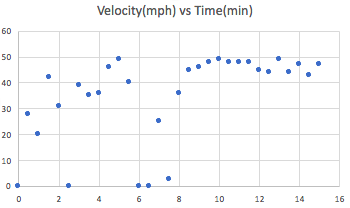
\includegraphics{scatter}
\begin{center}
    This is the scatterplot with the x-axis in time in minutes and the y-axis in velocity in miles per hour. 
\end{center}\\
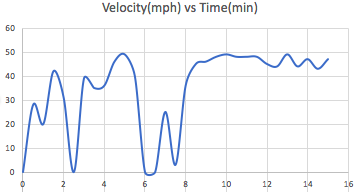
\includegraphics{graph}
\begin{center}
    This is the graph with the x-axis in time in minutes and the y-axis in velocity in miles per hour. 
\end{center}\\
\section{Analysis}
Percent Error\\
1. Percent Error for Midpoint Formula\\
$$\frac{\mid8.567-8\mid}{8}\cdot100= 7.088\%$$\\
2. Percent Error for Trapezoidal Method
$$\frac{\mid9.058-8\mid}{8}\cdot100= 13.225\%$$\\
The difference between the odometer readings and the calculations is noticeable. The odometer readings aren't completely inaccurate because the readings express the total mileage without a decimal. Therefore, the car could have traveled anywhere between 8 and 9 miles.\\\\
Overall, the trapezoidal method is an overestimate of the amount of miles traveled because the graph tends to increase. The midpoint formula is also inaccurate because both the midpoint and trapezoidal methods assume that the velocity is increasing or decreasing at a constant rate. In this case, the car wasn't increasing at a constant rate. So, in order to make this lab better, or more accurate, many more interval measurements would have to be taken.
\section{Summary}
During this project, three different methods of calculating the distance traveled over a 15 minute car ride were explored. The methods of calculating are not capable of taking irregular driving conditions such as red lights or turns into consideration. For this reason and others previously explained, none of the explored methods are fully accurate.
\end{document}
